%%document preambel

\documentclass{scrartcl}
\usepackage[ansinew]{inputenc}
\usepackage[T1]{fontenc}
\usepackage{graphicx}
%\usepackage{beramono}% monospaced font with bold variant

%\usepackage{listings}
%\lstdefinelanguage{VHDL}{
%  morekeywords={
%    library,use,all,entity,is,port,in,out,end,architecture,of,
%    begin,and
%  },
%  morecomment=[l]--
%}
%
%\usepackage{xcolor}
%\colorlet{keyword}{blue!100!black!80}
%\colorlet{comment}{green!90!black!90}
%\lstdefinestyle{vhdl}{
%  language     = VHDL,
%  basicstyle   = \ttfamily,
%  keywordstyle = \color{keyword}\bfseries,
%  commentstyle = \color{comment}
%}


\begin{document}

\title{Partial reconfiguration and fault simulation with Altera Cyclone fpga}
\subtitle{Students project at the chair of computer architecture university freiburg}
\author{Markus Wei�}
\maketitle
\tableofcontents
\newpage

\section{Software prerequisites}
The software used in both projects were Quartus II Version 14.1/15.0 and QSYS on Windows 7/8.1.\\Quartus II was needed to generate VHDL- or Verilog files which were used by a fpga (field programmable gate array). The Quartus II software can be configured to reach different design goals, e.g. time complexity, speed, optimization of compilation time or energy consumption.\\ QSYS is described as a tool for system integration, to safe time by generating automatic connection-logic for different components. The developed VHDL code from Quartus II software can be imported to QSYS and is processed there to connect different components on the dev kit board. QSYS has to initiate, configure and connect the hps (hard processor system) to the fpga if they need to communicate.\\ In addition to the development software some driver have to be installed on the running operating system. To program the fpga via the usb cable a special driver from altera needs to be installed. The installation of the Altera USB Blaster driver was not so intuitive as expected (see problems).\\
The following revisions and version of the software is used:
\begin{itemize}
	\item Windows 7/8.1 	
	\item Quartus II (Version 14.1/15.0)
	\item QSYS
	\item Altera USB Blaster driver
\end{itemize}
\newpage
\section{Partial reconfiguration}
\subsection{Prerequisites}
The \textbf{hardware} used for this project was a development kit board from altera, namely "Terasic DE1-SoC Development Kit". This board consist of the following core components: a FPGA, named Altera Cyclone V FPGA (5SCEMA5F31C6N), a dual-core Cortex-A9 (HPS), 1GB DDR3 and 64MB SDRAM and different interfaces (USB,JTAG,i2c). The communication interfaces are a on board USB-Blaster II, USB 2.0 ports, UART interface, Ethernet port and extended module for gpio pins.\\
The fpga is the mainly used component of the development kit board. Here are some useful facts about the fpga Cyclone V:\\
\begin{itemize}
	\item 85000 logic cells on the board
	\item 4450 kb embedded memory
	\item access to an external 64 MB static random access memory (SRAM)
	\item low energy consumption
\end{itemize}
The Cyclone V is configured through the USB Blaster interface, where a bit stream is loaded to the memory of the board. This bit stream is lost once the energy is off. Alternatively an in-system NOR flash memory, which safes the bit stream while power is taken off, can be loaded with this bit stream.\\ Another way to program the fpga is to use the hard processor system (hps). This is done either while the boot process with "U-Boot" or the "preloader" or after the operating system is fully booted.\\ The \textbf{preloader} initiates the clock, is responsible for multiplexing pins, configures the main memory and loads the U-Boot.  The configuration of the main memory of the hard processor system and the AXI Bridges is crucial, because these have to grant the fpga access.\\ The \textbf{universal boot loader} initiates and tests hardware components. Also it downloads and executes application software. This boot-loader is required to initiate the boot process of the UNIX-kernel. \\ The \textbf{Avalon-Memory-Mapped-Interface} enables efficient read- and write operations, interrupts, clocks, resets and control progresses. This Avalon-MM-Interface enables address based read- and write procedures in a master/slave connection. The master put a request to the slave, which read or write special addresses of the memory. This interface is required to get access from the FPGA to the main memory of the HPS.\\ To work with an external C/C++ program an operation system for the hps is needed. The chosen OS is a linux system.
\subsection{The idea and the benefit}
The concept of partial reconfiguration is highly desirable for some special purposes. With this feature it would be easier to change partially designs or improve the functionality of a fpga without interrupting its work progress. Special applications need to change some logic on a fpga while another part of the fpga is not allowed to stop. For example the flow of data should not be stopped while another part is changing something. Therefore this concept is desirable in the field of communication systems. A benefit of this idea is that the number of devices can be scaled down, therefore the power consumption and of course the cost. The tasks another fpga has handled before can now be handled by the same fpga, only another part of the logic cells take it. \\Thanks to this feature the fpga can handle a new input while another part still executes its commands.\\
This reconfiguration is either initialized by an external host or an internal one. With the internal host, a processor on the development kit (hps)  initializes the process and starts to program the desired locig cells of the fpga while the other part remains in its process. This initiation is done by an internal host which runs a C/C++ program. This C/C++ program is stored in the RAM (read access memory) of the development kit board.\\
Partial reconfiguration could be combined with the fault simulation on fpga for an efficient way to detect logic errors.

\subsection{Design flow and implementation}
The focus of the partial reconfiguration is rather on logic blocks than DSP, memories, PLL, transceivers and I/O blocks. Functions in the periphery like GPIO or I/O registers can not be partially reconfigured.\\ 
For the partial reconfiguration of logic blocks two different regions in the top level design are needed.
One static region, which continues the initialized process and one region, which can be reconfigurated on the fly.
To get an optical feedback of this configuration process, two led pattern are generated. One pattern, in the static region, highlights the leds to check if the fpga is still running while another led pattern is loaded to the dynamic or partial reconfiguration region which let us check if a part of the fpga is reconfigured.\\
To avoid in- and output errors while reconfiguration, a wrapper region is needed. This region is generated to ensure that all personas, e.g. led pattern, have the same connection to the static region. 
This is done by creating dummy ports.\\
For partial reconfiguration all non-global inputs of the pr regions must be freezed. Freezing means in this context to drive a '1' to the inputs, which ensures there is no contention between current values and those after partial reconfiguration. Therefore a freeze region is essential.\\The projects idea was a partial reconfiguration with an internal host, which initializes the reconfiguration with a c/c++ program. To do so, the processor has to communicate with the fpga and with the memory. The communication between the hard processor system and  the fpga, the main memory and in- and output interfaces is a crucial point.\\  The design flow used in this project:
\begin{enumerate}
	\item planning the system for partial reconfiguration
	\item identify which blocks to be partially reconfigured $\rightarrow$ led pattern for the led on DE1-SoC board
	\item code the design in Quartus II
	\item develop the personas
	\item generate static and pr region
	\item assign partitions to logiclock regions
	\item create necessary files to program fpga
	\item program fpga 
\end{enumerate}
The fpga development process is done by Quartus II and QSYS. Quartus II creates the FPGA components in VHDL, while QSYS connects different system components which communicate and access each other. This informations are required to generate the "preloader" which coordinates the boot process. The next step of booting is the "universal boot loader" which configures the fpga and load the "linux-kernel". The Avalon-MM-Interface is required to grant the fpga access to the main memory of the HPS.\\

%Two different led pattern, a wrapper and a freeze region were designed. The design partition were associated with the logiclock regions of the fpga
%	\item connect I/O signals with pins (QSYS)


%There are different options for the communication between HPS and FPGA, which are mentioned here without a detailed description. 
%\begin{enumerate}
%	\item Advanced extensible interface bus bridges (AXI)
%	\begin{enumerate}
%		\item Lightweight HPS-to-FPGA bridge
%		\item HPS-to-FPGA bridge
%		\item FPGA-to-HPS bridge
%	\end{enumerate}
%	\item FPGA-to-SDRAM
%\end{enumerate}

%\\ Project design flow, hierarchy etc, code citation.
%Which design blocks are necessary to program the fpga for partial reconfiguration. Wrapper, logic, etc. ...comment on created code.

\subsection{Problems}
There occurred two crucial problems during the work on partial reconfiguration.
\begin{enumerate}
	\item  No permission to use partial reconfiguration feature in Quartus Software
	\begin{itemize}
		\item a new license was inquired
	\end{itemize}
	\item the fpga Cyclone V does not support the feature of partial reconfiguration
	\begin{itemize}
		\item could not be solved because a new special fpga was not affordable
	\end{itemize} 
\end{enumerate}
After working 8-10 weeks on this topic the project has to be stopped due to the fact that partial reconfiguration is not supported by the cyclone V fpga. At this time the status quo was:
\begin{itemize}
  \item literature survey
  \item soft- and hardware prerequisites
  \item project design flow
  \item creating different revisions for partial reconfiguration in Quartus II
  \item VHDL design
	\begin{itemize}
		\item top level
		\item wrapper
		\item freeze region
		\item static region + personas
		\item partial reconfiguration region + personas
	\end{itemize}
  \item pin assignments
  \item file creation for programming the fpga (.pmsf, .msf, .sof, .rbf)
\end{itemize}
Researching on this topic of partial reconfiguration it worth it. Partial reconfiguration can be used in time critical systems, like communication systems, where an abrupt stop of a data flow is critical. The field of partial reconfiguration is still a new topic for researcher and yet it is not integrated in industrial products. The main disadvantage is the cost of a special fpga instead of using an cheaper ASIC and a lot more time must be spent on validation.
\newpage
\section{Fault simulation}
\subsection{Prerequisites for the project of fault simulation}
The \textbf{hardware} used in this part of the project was a former dev kit from altera with a fpga Cyclone IV.\\
In addition to the software mentioned in section 1, there is some \textbf{special software} required for this part of the project:
%In addition to the mentioned software in the beginning some special software is required:
\begin{itemize}
	\item C++ compiler e.g. MinGW $\rightarrow$ compile C++ file to *.exe file
	\item USB-to-Serial driver $\rightarrow$ get a connection for communication purpose from dev kit to pc via RS232
\end{itemize}
Also a couple of files from a former project of two students were provided.
\subsection{Idea of fault simulations in hardware}
The idea of fault simulation is to detect stuck-at faults with the fpga. A special test pattern is loaded to the ram of the fpga. This is done by the communication from pc to the fpga via usb blaster. The circuit under test is realized by one circuit without fault pattern and one with changed lcells. The changed logic cells are loaded with test pattern to compare both. The output of both circuits is lead to a logical XOR gate. If the outputs of both circuits distinguishes the XOR gate give a logical one, hence a fault. Otherwise no fault is detected. This output is saved in a fifo and then transmitted to the pc for documentation purposes via the serial interface RS232.
%Efficient fault simulation in hardware FPGA. modification of the circuit with special changes to the look up tables. evaluation and pc communication with serial interface rs232.\\
%To detect faults some lcells are modified. 
% \textbf{lcell}
% \begin{itemize}
%	\item smallest logic cell
%	\item maximal four inputs
%	\item gatter are ordered in a logic cell
%	\item every lcell have a look-up table, which defines the output
%	\item the function of a particular  lcell can be changed by hand
%\end{itemize}
The idea of the Maximum fanout free cones (MFFC), adopted from a former project,   is to assign as many as possible gates to one logic cell. The creation of maximum fanout free cones is an algorithm to minimize the number of gates in one logic cell. This algorithm is implemented in quartus by a former work. The original circuit under test is compared to a modified circuit. The look-up table (LUT) can be calculated for every locig cell in quartus. The idea of the fault injection test is an efficient way to detect faults in hardware. The evaluation is done over the rs232 interface and a personal computer. The goal is a very fast way to detect those faults.


\subsection{preparation and process to execute the fault simulation on the development kit}
After setting up the software prerequisites you have to change the absolute paths  inside the C++ files to the desired programs. This list shows the process to execute the fault simulation on the fpga: 
\begin{enumerate}
	\item compile quartus project
	\begin{itemize}
		\item open 'FaultInjectionTester.qar' with Quartus II
		\item compile this project
		\item close Quartus II
	\end{itemize}
	\item create IRA.exe in root folder (make.batch file)
	\begin{itemize}
	\item open command window and change directory to FaultConfiguration
	\item execute: \textit{g++ IRA.cpp CGate.cpp CGate.h CComponent.h -o ..IRA.exe}	
	\end{itemize}
	\item create FaultInjectionTester.exe in root folder (make.batch file)
	\begin{itemize}
	\item open command window and change directory to FPGACommunication
	\item execute: \textit{g++ FaultInjectionTester.cpp PcFPGACommunication.cpp PcFPGACommunication.h -o .."FaultInjectionTester.exe"}
	\end{itemize}
	\item Connect board and pc via USB Blaster
	\item connect board and pc via RS232
	\item execute IRA.exe [path to quartus], e.g. IRA.exe "C://Program Files//Altera"
\end{enumerate}
If it all worked well, the pc programs and tests the fpga. The communication link is via the RS232 interface, for which the usb to serial driver is necessary.\\
Otherwise following common errors can occur while executing:
\begin{itemize}
	\item "Inconsistent set or reset compile started variable" $\rightarrow$ clear out "db" and "incremental\textunderscore db" folder in "FaultInjectionTester\textunderscore restored" folder and recompile quartus project
	\item "Can not find quartus\textunderscore cdb" $\rightarrow$ you have to change the HDD constant in FPGACommunication/PcFPGACommunication.cpp and FaultConfiguration/IRA.cpp to the drive where your quartus is installed.
\end{itemize}

%explain the complete process:
%\begin{enumerate}
%	\item TCL script
%	\item batch
%	\item quartus project
%	\item c++ files
%	\item exe files
%	\item vhdl files
%\end{enumerate}

\subsection{Implementation}
First of all the execution of the c compiler by hand was enhanced. A batch file was created which can be executed without wondering which command has to follow which on which workspace. This was the first step to set up the project for everyone desire. The second step was to change absolute paths to relative paths, which also makes the project better for other working machines. Then a huge error was detected in the design flow. This shows that the previous work was not fully completed if nobody could find this fault before. This makes it difficult to work proper with this project.  A bunch of weeks was wasted on debugging and struggling with several software installation problems to run this project. Which create the idea of redo the whole project and setting it up to an independent state, so that everybody can use it without special requirements. This idea is based on a virtual machine with version control. Also only the really needed files were imported so the project structure is still remarkable, recognizable. This short instruction should be good start for future works on this project.
\subsection{Problems}
Debugging and to solve problems on installation and design flows become the main part of the project work. Here are the problems which occur during the project.
\begin{enumerate}
	\item driver installation of USB blaster II and FTDI Chip for USB-Serial converter
	\item error in design flow
	\item error while execution: inconsistent set and quartus could not be fond
\end{enumerate}
Also it seems to be intuitive to install a USB driver, it was quite difficult to install under Win 8.1 because the delivered driver has no driver signature which is required for Win 8.1. To install a driver without signature you have to follow these steps to install it anyway. First of all i encountered the problem of driver installation. Although it seems to be trivial, if you encounter this problem: 
\begin{figure}[ht]
	\centering
  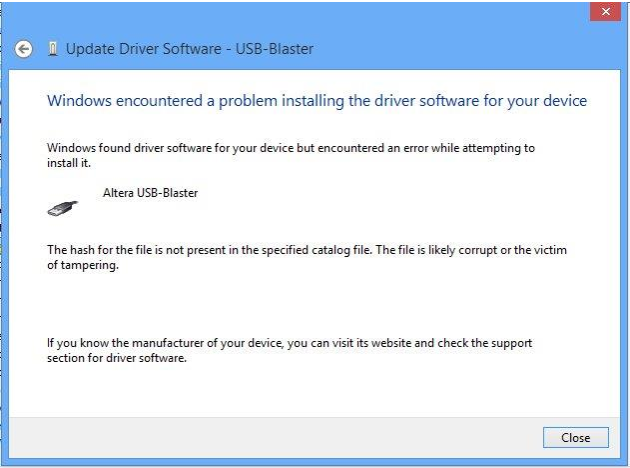
\includegraphics[width=0.8\textwidth, angle=0]{USB_blaster_driver_problem.png}
	\caption{failed installation of usb blaster driver}
	\label{usbblasterproblem}
\end{figure}
you have to follow these steps to install the usb driver:

\begin{figure}[ht]
	\centering
  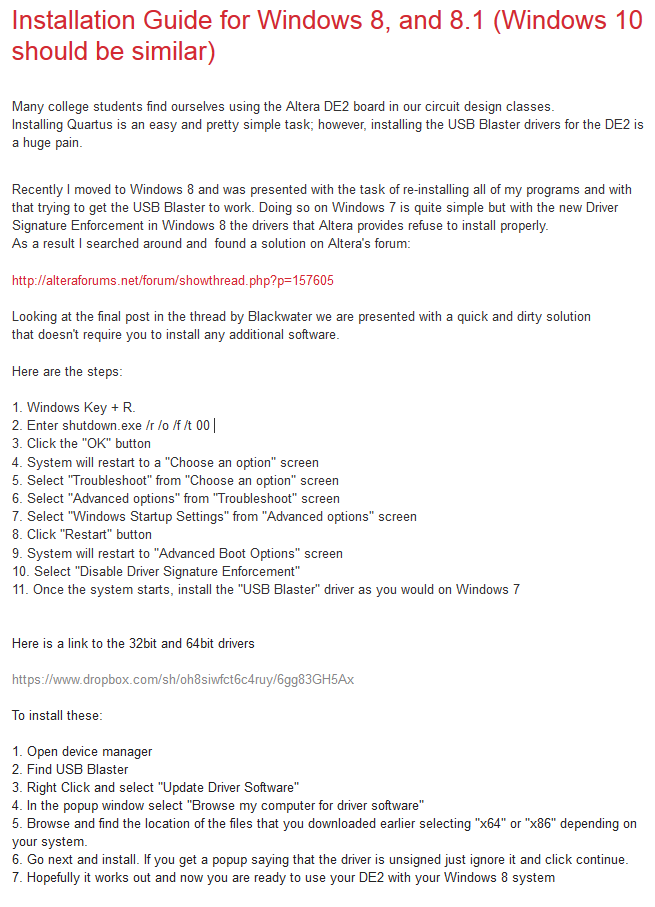
\includegraphics[width=1\textwidth, angle=0]{installationGuide.png}
	\caption{steps to install the usb driver}
	\label{installguide}
\end{figure}
Although it is an official driver from altera i was struggling with this problem a few days to find out, that windows 8.1 does not support this official driver. The solution is found on: \textbf{\textit{http://altera-guide.blogspot.de/2012/11/many-collage-students-find-ourselves.htmlcomment-form}} \\
%The solution for the inconsistent set error would be to clear out 'db' and 'incremental db' in 'FaultInjectiontester restored' folder and recompile the quartus project.\\
%If a 'quartus' execution file could not be found, you have to check the paths entered in FPGACommunication.cpp and IRA.cpp and change them. \vspace{1cm}
A lot of problems occurred during this work. These problems prevented that vhdl could be learned, which was the intend to do a project at the chair of computer architecture. The second project was nearly only a project in the programming language of C++ and no more hardware programming.
The workstation for this project was my desktop pc and not my laptop, so this makes it difficult to share the problem among the other guys. The best way to enhance this project were to redo the whole project. The idea was to set up a whole new project which runs fine on my machine but then it would run fine on my work station but not in common. So there would be a good improvement, to set up a virtual machine with software which runs independent of the users operating system. There would be only one supported software version of Quartus II and QSYS, the driver could be set up once. This setup would have taken too much time in the workload of this project.
This took a very long time, because it is so complicated and not documented and not trivial. Also there was a huge error in the design flow, which took very long to detect. 
Than there was the problems discussed earlier. 
Debugging and troubleshooting become the main part of the project.\\
The improvements and changes which were made:
\begin{itemize}
	\item changed absolute paths to relative paths
	\item code debugging
	\item error in design flow detected: re-compilation after changing the LUTs is missing
	\item create a batch file to automate process
\end{itemize}
Further improvements for future work is to setup the program on a virtual machine to become independent of operating system and thus driver installation. Also a version control for this program would be great for future works and a nice structure of the project. In this project is no structure and it makes it very difficult to understand whats going on.\\

% path to installed software. troubleshooting for installation of usb blaster driver. debugging former code fractions. error in design flow (compilation missing after changing luts). creating batch file to automate it. relative paths to automate. further improvements: design for a virtual machine, version control. 
%All in all i can say to work on a proper design is very difficult.
%The communication link between RS232 and Board work properly, but without the information on the Version of used software (quartus, qsys, operating system etc.) it is too difficult.
%Also the installation path should not be absolute.
%%There were an error that the project was not compiled after changing the LUTs. 
\newpage
\section{Appendix}
\subsection*{Problems and Errors}
\begin{figure}[ht]
	\centering
  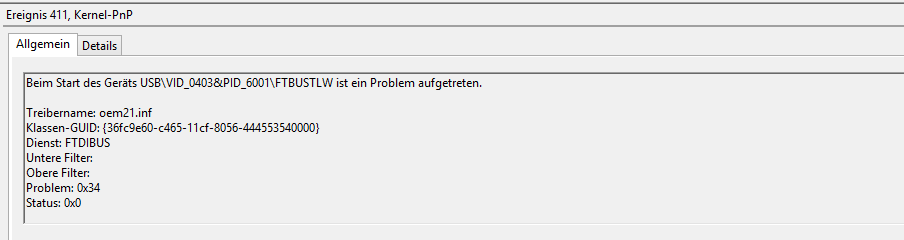
\includegraphics[width=1\textwidth, angle=0]{FTDI_USB_SERIAL_CONVERTER_problem.png}
	\caption{FTDI chip problem}
	\label{ftdi_problem1}
\end{figure}

\begin{figure}[ht]
	\centering
  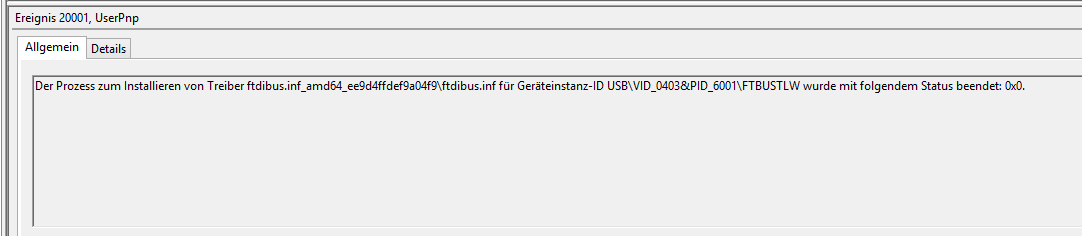
\includegraphics[width=1\textwidth, angle=0]{FTDI_USB_SERIAL_CONVERTER_problem2.png}
	\caption{Driver install not successful}
	\label{ftdi_problem2}	
\end{figure}

\begin{figure}[ht]
	\centering
  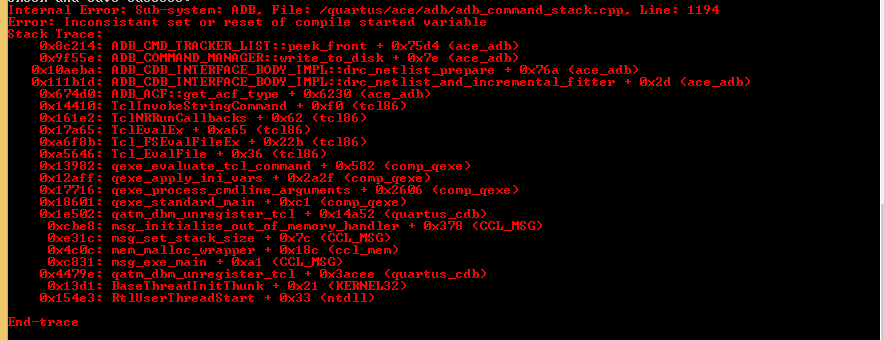
\includegraphics[width=1\textwidth, angle=0]{inconsistent_set.png}
	\caption{inconsistent set}
	\label{inconsistentset}	
\end{figure}

\begin{figure}[ht]
	\centering
  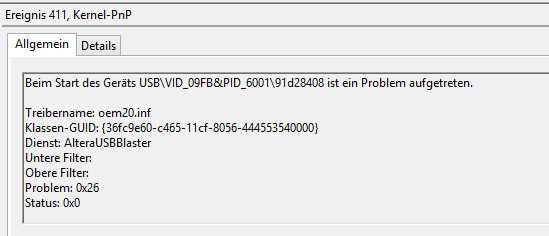
\includegraphics[width=1\textwidth, angle=0]{USB_blaster_problem.png}
	\caption{AlteraUSBBlaster problem}
	\label{usbblaster1}	
\end{figure}

\begin{figure}[ht]
	\centering
  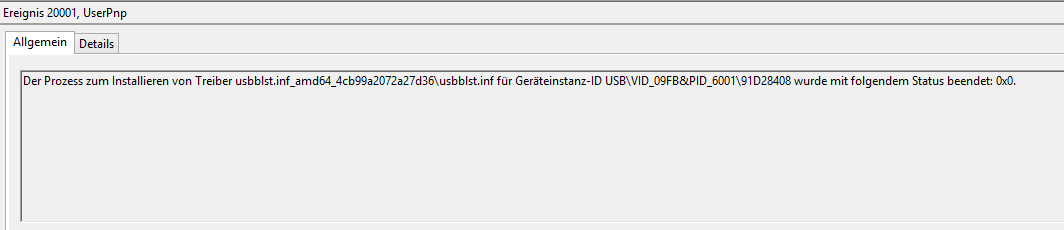
\includegraphics[width=1\textwidth, angle=0]{USB_blaster_problem2.png}
	\caption{AlteraUSBBlaster install not successfull}
	\label{usbblaster2}	
\end{figure}

\begin{figure}[ht]
	\centering
  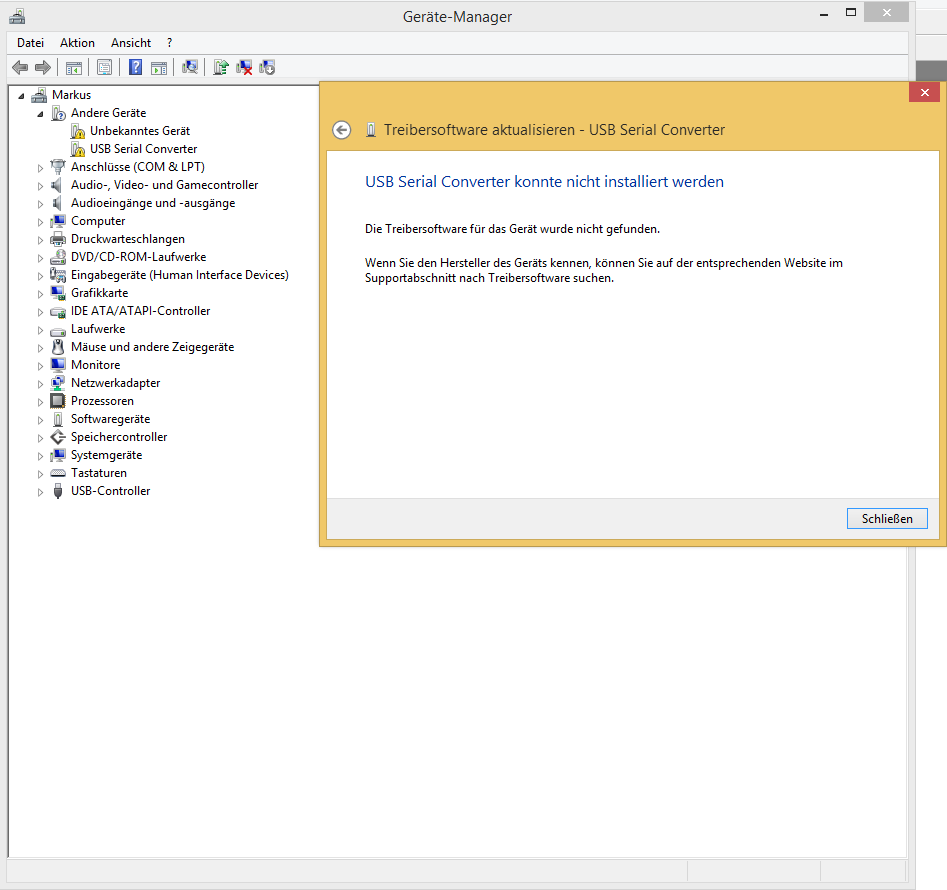
\includegraphics[width=1\textwidth, angle=0]{USB_serial_driver.png}
	\caption{USB Serial Converterter could not be installed}
	\label{usb_serial_problem}	
\end{figure}
% \section{Appendix - VHDL Code}
\subsection{PR top level}
\begin{lstlisting}[style=vhdl]
library IEEE;
use IEEE.std_logic_1164.all; 

entity PR_test_top is
    port( 
     
            --Button to start PR
            PR1_button          : in STD_LOGIC;

            
            --DIP switch to select PR_bitstream
            dir_switch_1        : in STD_LOGIC;
            
            --DIP switch to change blinking mode 
            dir_switch_2        : in STD_LOGIC;
            
            
            system_clock        : in STD_LOGIC;
            PR_reset_button : in STD_LOGIC;
            
            PR_done_led         : out STD_LOGIC; 
            PR_error_led        : out STD_LOGIC;            
            LED                 : out STD_LOGIC_VECTOR (3 downto 0);
            -- 7 segment display
            disp_hex0           : out STD_LOGIC_VECTOR (6 downto 0);  
            disp_hex1           : out STD_LOGIC_VECTOR (6 downto 0);
            disp_hex2           : out STD_LOGIC_VECTOR (6 downto 0);
            disp_hex3           : out STD_LOGIC_VECTOR (6 downto 0);
            disp_hex4           : out STD_LOGIC_VECTOR (6 downto 0);
            disp_hex5           : out STD_LOGIC_VECTOR (6 downto 0)
        );
            
end PR_test_top;

architecture behv of PR_test_top is
    component freeze_region
         port( clk          :in STD_LOGIC;
            dir             :in STD_LOGIC;       
            freeze          :in STD_LOGIC;
            leds                :out STD_LOGIC_VECTOR (3 downto 0)
            );
    end component freeze_region;
     
    component pr_user_host is
    port(   areset          : in STD_LOGIC;
             clk                    : in STD_LOGIC;
             channel            : in STD_LOGIC;
             allow_pr_start : in STD_LOGIC;

              -- Outputs
             testing_done       : out STD_LOGIC; 
             pr_freeze          : out STD_LOGIC; 
             error_flag_pr  : out STD_LOGIC; 
             really_done        : out STD_LOGIC);
    end component pr_user_host;
    
    component ticker_disp is
         port( clk                  : in STD_LOGIC;
                disp_hex0           : out STD_LOGIC_VECTOR (6 downto 0);
                disp_hex1           : out STD_LOGIC_VECTOR (6 downto 0);
                disp_hex2           : out STD_LOGIC_VECTOR (6 downto 0);
                disp_hex3           : out STD_LOGIC_VECTOR (6 downto 0);
                disp_hex4           : out STD_LOGIC_VECTOR (6 downto 0);
                disp_hex5           : out STD_LOGIC_VECTOR (6 downto 0)
            );
    end component ticker_disp;
    
    -- ****************** Missing ***********************
    --  component for LED 3-0
    -- clk                  : in STD_LOGIC;
    --  LED                 : out STD_LOGIC_VECTOR (3 downto 0));

    
--signal max_count:integer  := 300000000;       -- 08.06.2015 Ticker
--signal count:integer      :=0;                    -- 08.06.2015 Ticker
signal pr_freeze_reg        : STD_LOGIC;
signal pr_freeze                : STD_LOGIC;
signal channel              : STD_LOGIC;
signal done_w                   : STD_LOGIC;
signal really_done          : STD_LOGIC;
signal error_flag_pr_w      : STD_LOGIC;
     
begin 
channel <= dir_switch_1;
 
freeze_region_inst: freeze_region
 port map (
   clk      => system_clock,
   freeze   => pr_freeze_reg,   
   dir      => dir_switch_2, 
   leds     => LED(3 downto 0)

    );

pr_user_host_inst : pr_user_host    
port map (
      areset         => PR_reset_button,
      clk            => system_clock,
      testing_done   => done_w,
      pr_freeze      => pr_freeze,
      error_flag_pr  => error_flag_pr_w,
      allow_pr_start => PR1_button,
      channel        => channel,
      really_done    => really_done);

ticker_inst: ticker_disp
 port map (
   clk         => system_clock,
    disp_hex0   => disp_hex0,   
    disp_hex1   => disp_hex1,   
    disp_hex2   => disp_hex2,   
    disp_hex3   => disp_hex3,   
    disp_hex4   => disp_hex4,   
    disp_hex5   => disp_hex5
   );
 
 process(system_clock) begin
    if rising_edge(system_clock) then
        PR_done_led         <= not done_w; 
        pr_freeze_reg     <= pr_freeze;     
        PR_error_led        <= not error_flag_pr_w;
    end if; 
end process;

        
end behv;

\end{lstlisting}

\end{document}
